\chapter{Estudio espectral de los polinomios discretos de Legendre}
\label{chap: estudio espectral}

No es difícil convencerse de que las condiciones de ortogonalidad
impuestas en la definición de la base de discreta de Legendre
$\cali{L}^{n}$
forzan a las entradas de los polinomios discretos $\cali{L}^{n,k}$
a cambiar más frecuentemente de signo conforme aumenta
el grado $k$, luego, conforme $k$ tiende a $n-1$,
la cantidad de oscilaciones aumenta; revisemos, 
por ejemplo, el caso $n=4$.



\begin{minipage}{0.5\textwidth}
\begin{figure}[H]
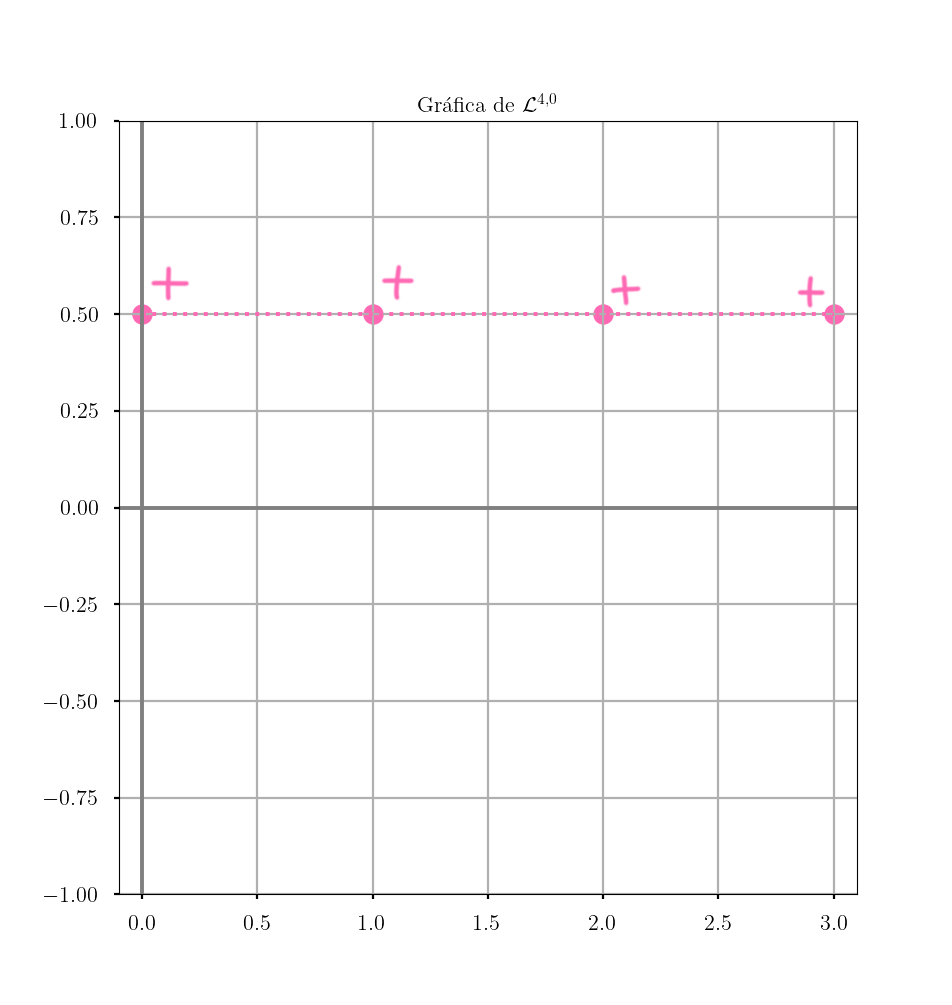
\includegraphics[scale=0.25]{oscil1}
\end{figure}
\end{minipage} \hfill
\begin{minipage}{0.45\textwidth}
1.- Por definición,
$\mathcal{L}^{4,0}$ se obtiene al normalizar 
al vector constante uno de $\IR^{4}$, o sea, 

\[
\cali{L}^{4,0} = \left(
\frac{1}{2}, \frac{1}{2}, \frac{1}{2}, \frac{1}{2}
\right).
\]
\end{minipage} 


\begin{minipage}{0.5\textwidth}
2.- La señal $\cali{L}^{4,1} \in \IR^{4}$ es un polinomio discreto de
dimensión 4 y grado 1 que se obtiene exigiendo las
siguientes condiciones

\[
\langle \cali{L}^{4,1} , \cali{L}^{4,0} \rangle=0
\hspace{0.2cm} \text{y} \hspace{0.2cm}
\langle \cali{L}^{4,1} , \cali{L}^{4,1} \rangle=1;
\]
esta primera condición se refleja en que 
las alturas de los puntos de la gráfica de 
$\cali{L}^{4,1}$ deben sumar cero;
esto implica un cambio de signo (y sólo uno,
pues el polinomio es lineal).

\end{minipage} \hfill
\begin{minipage}{0.45\textwidth}
\begin{figure}[H]
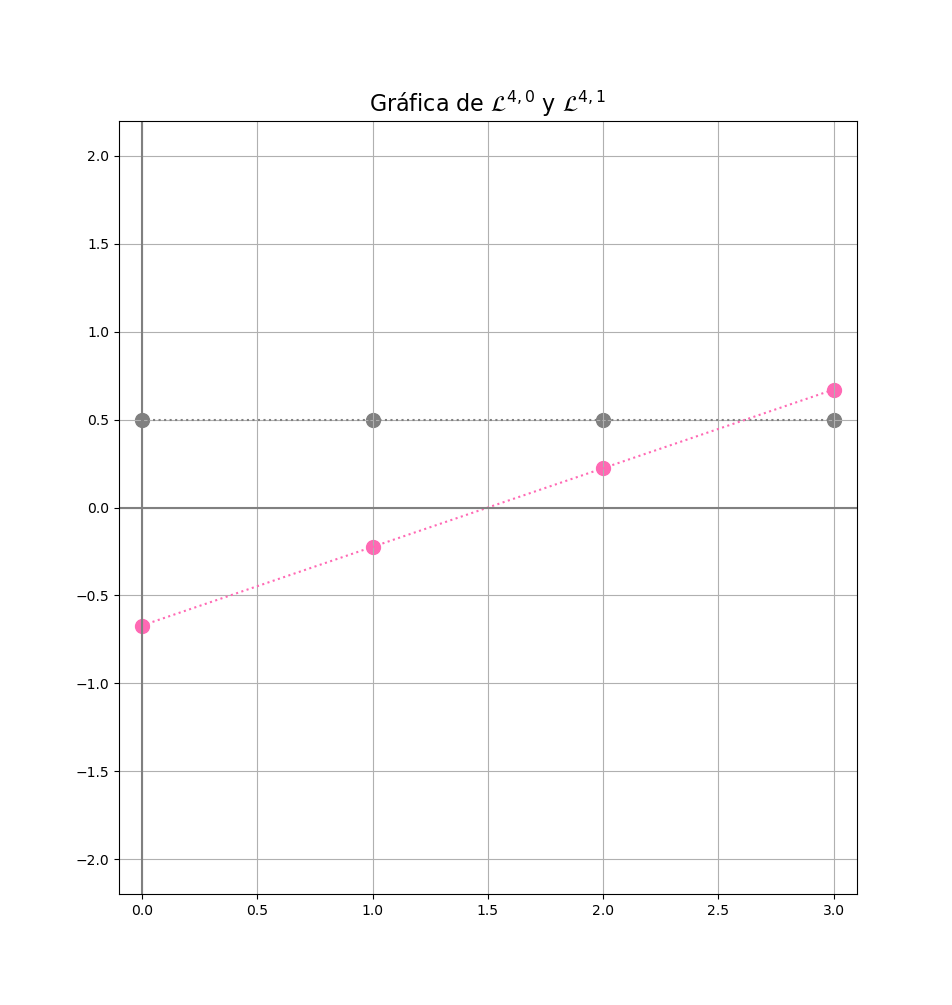
\includegraphics[scale=0.3]{oscil2}
\end{figure}
\end{minipage}

\noindent
3.- El vector
$\cali{L}^{4,2} \in \IR^{4}$ satisface las siguientes
tres condiciones:

\[
\langle \cali{L}^{4,2} , \cali{L}^{4,0} \rangle=0,
\hspace{0.2cm}
\langle \cali{L}^{4,2} , \cali{L}^{4,1} \rangle=0,
\hspace{0.2cm} \text{y} \hspace{0.2cm}
\langle \cali{L}^{4,2} , \cali{L}^{4,2} \rangle=1;
\]
observe que si las entradas de 
$\cali{L}^{4,2}$ fuesen todas positivas o todas negativas,
entonces no se tendría la ortogonalidad
con la señal constante $\cali{L}^{4,0}$.


\begin{figure}[H]
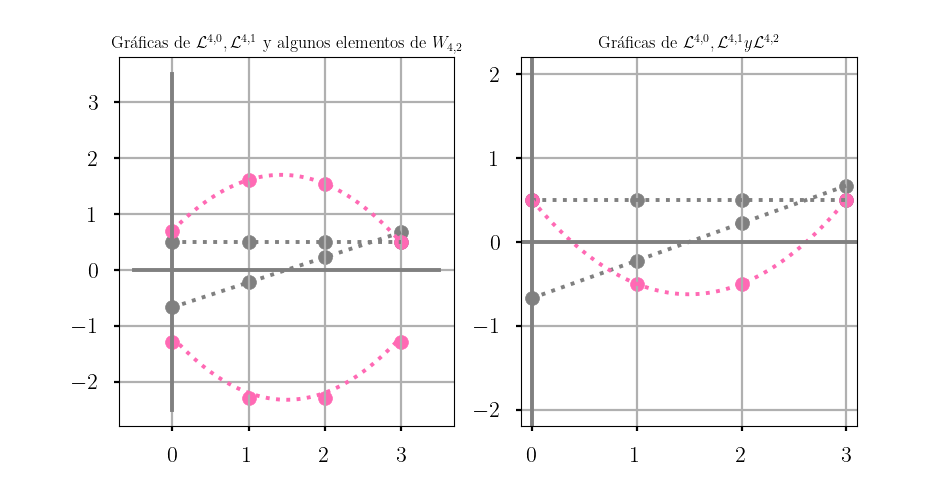
\includegraphics[scale=0.6]{oscil3}
\end{figure}

4.- Por último, $\cali{L}^{4,3} \in \IR^{4}$ satisface
las siguientes cuatro condiciones: 

\[
\langle \cali{L}^{4,3} , \cali{L}^{4,0} \rangle=0,
\hspace{0.2cm}
\langle \cali{L}^{4,3} , \cali{L}^{4,1} \rangle=0,
\langle \cali{L}^{4,3} , \cali{L}^{4,2} \rangle=0,
\hspace{0.2cm} \text{y} \hspace{0.2cm}
\langle \cali{L}^{4,3} , \cali{L}^{4,3} \rangle=1.
\]

Según los teoremas 
\ref{cor: propiedades importantes de espacios Wi}
y \ref{prop: simetrias en dimensiones pares},
$\cali{L}^{4,3}$ es la discretización de un polinomio
cúbico y además es una señal antisimétrica (en el sentido de la definición
\TODO{ref}); dos gráficas de señales que cumplen esto se ilustran abajo:

\begin{figure}[H]
	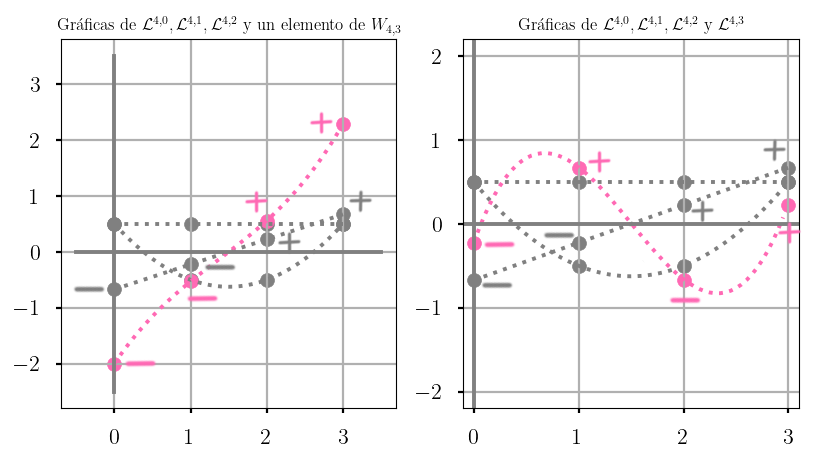
\includegraphics[scale=0.6]{oscil4}
	\sidecaption{Observe que la señal cúbica de la izquierda tiene
	un sólo cambio de signo, mientras que la de la derecha (que es 
	$\cali{L}^{4,3}$ tiene tres.)}
\end{figure}

La señal cúbica de la izquierda, a pesar de 
ser ortogonal a $\mathcal{L}^{4,0}$ y a $\cali{L}^{4,2}$ por 
simetría (c.f. lema
\ref{lema: ortogonalidad entre sim y antisim}), 
definitivamente no puede ser ortogonal
a $\cali{L}^{4,1}$, pues las entradas de estos dos vectores de 
$\IR^{4}$ tienen el mismo signo. Sin embargo, la señal cúbica 
de la derecha (que de hecho es $\cali{L}^{4,3}$) sí cumple el ser
ortogonal a $\cali{L}^{4,1}$ pero, para lograr esto, sus
entradas deben cambiar de signo tres veces.

\TODO{Recuerda que también debes de decir que importa el orden
creciente de los grados; si hubieses definido primero a l2, entonces no necesariamente tendrías tantas oscilaciones.}

\subsection{Estudio de presencia de frecuencias particulares via mediciones de distancia a espacios de frecuencia}

Queremos ahora generalizar el estudio anterior y no restringirnos
al estudio de frecuencias enteras, \TODO{Aquí dí por qué}
sino el poder elegir una frecuencia $\omega \geq 0$ respecto
a la cual comparar a la señal. A pesar
de que ya no contaremos con la seguridad de trabajar con bases
ortonormales de $\IR^{n}$, queremos considerar espacios de frecuencias
en base a los cuales medir la distancia de $x$ a estos, siendo
esta una medida de qué tanto reacciona $x$ a la frecuencia $\omega$.
\TODO{Cita el ejemplo en el que haces esto para medir qué tan afín es
una señal.}

Antes de empezar, 
\sidenote{Para simplificar la notación, denotamos por $I_{n}$ al intervalo
$\{ \frac{\mu }{n}  : 0 \leq \mu \leq n-1 \}$.}
digamos qué es lo que 
entendemos por ``señales de frecuencia pura''.
\begin{defi}
Sean $n \in \IN$,  $\omega>0$, $\phi \in [0,1]$.  A toda señal $n-$
dimensional  
de la forma

\begin{equation}
A \left(
cos \left(  2 \pi \omega t + 2 \pi \phi
\right)
\right)_{t \in I_{n}}
\end{equation}
y

\begin{equation}
A \left(
sin \left(  2 \pi \omega t + 2 \pi \phi
\right)
\right)_{t \in I_{n}},
\end{equation}

\noindent
con $A \in \IR$, se le llamará
\textbf{señal $n-$dimensional de frecuencia
pura $\omega$}. En este contexto,
a $\phi$ se le llama el \textbf{desfase normalizado}
de la señal, y a $A$ la \textbf{amplitud}.
\end{defi}
\TODO{Aquí deberías de poner una figura en la que enseñes que para formar
a estos vectores muestreas uniformemente sinusoides.}


\begin{defi}
Sean $n \geq 2$ es un entero y $\omega \geq 0$ un número no negativo.

Si $n$ divide a w, definimos a los siguientes vectores de $\IR^{n}$
\begin{equation}
\label{eq0: 27Marzo23}
f_{n, \omega} = \left( 
\frac{1}{\sqrt{n}}, \ldots , \frac{1}{\sqrt{n}}
\right) \in  \IR^{n}
\end{equation}
y
\begin{equation}
\label{eq1: 27Marzo23}
g_{n, \omega} = \left( 
0,  \ldots , 0
\right) \in \IR^{n}.
\end{equation}

En caso contrario, definimos a los vectores

	\begin{equation}
	\label{eq5: 19Marzo}
	f_{n, \omega}= \left( \xi_{n, \omega} cos \left(2 \pi \omega \frac{\mu }{n} \right) \right)_{0 \leq \mu \leq N-1}
	\in \IR^{n}
	\end{equation}
y 

	\begin{equation}
	\label{eq6: 19Marzo}
	g_{n, \omega}= \left( \eta_{n, \omega} sen \left(2 \pi \omega \frac{\mu }{n}\right) \right)_{0 \leq \mu \leq N-1}
	\in \IR^{n},
	\end{equation}
donde

\begin{equation}
\label{eq7: 19Marzo}
	\xi_{n, \omega}= 
	\sqrt{2} \cdot \left( n + \frac{sen(2 \pi \omega)
	cos(2 \pi \omega \left( 1- \frac{1}{n} \right))}{sen \left(2 \pi 
	\frac{\omega}{n} \right)} \right)^{-\frac{1}{2}} 
\end{equation}
y

	\begin{equation}
	\label{eq8: 19Marzo}
	\eta_{n, \omega}= \sqrt{2} \cdot \left( n - \frac{sen(2 \pi \omega)
	cos(2 \pi \omega \left( 1- \frac{1}{n} \right))}{sen \left(2 \pi 
	\frac{\omega}{n} \right)} \right)^{-\frac{1}{2}}
	\end{equation}

\noindent	
les llamaremos los \textbf{vectores unitarios base de frecuencia $\omega$}.
\end{defi}


\begin{obs}
\label{obs: f y g son l.i. y de norma uno}
Sean $n \geq 2$ entero, $\omega >0$ con $n \nmid \omega$.
Si $f_{n, \omega}$ y $g_{n, \omega}$ son como en 
\eqref{eq5: 19Marzo} y \eqref{eq6: 19Marzo}, respectivamente,
entonces estos son vectores unitarios y linealmente independientes entre sí.
\end{obs}
\noindent
\textbf{Demostración.}

El que los
vectores $f_{n, \omega}$ y $g_{n, \omega}$ sean 
linealmente independientes
se deduce del que la primera entrada de $f_{n, \omega}$ no sea cero
mientras que la primera entrada de $g_{n, \omega}$ sea cero, pero no
todas sus entradas sean cero. 

Los números $\xi_{n, \omega}$ y $\eta_{n, \omega}$
mostrados en \eqref{eq7: 19Marzo} y \eqref{eq8: 19Marzo}
se definieron de tal forma que $f_{n, \omega}$ y $g_{n, \omega}$ tuviesen norma uno;
la forma de obtener a estos escalares de normalización de forma explícita fue
totalmente análoga a las operaciones que se realizan en la prueba de la proposición
\ref{prop: producto punto entre f y g}, por lo que omitimos los detalles.
\QEDB
\vspace{0.2cm}


Por ser $f_{n, \omega}$ y $g_{n, \omega}$ (cuando $n \nmid \omega$)
linealmente independientes, el espacio $P_{\omega}$ que generan

\begin{align}
\label{eq2: 20Marzo}
P_{\omega}:= & span(f_{n, \omega}, g_{n, \omega}) \notag  \\  
= &
\{ a \left( cos \left(2 \pi \omega t \right) \right)_{t \in I_{n}} +
b ( sen (2 \pi \omega t ))_{t \in I_{n}} : 
\hspace{0.2cm} a, b \in \IR \}. 
\end{align}

\noindent
es un plano \sidenote{O sea, un subespacio
de dimensión 2.} de $\IR^{n}$.
\TODO{Como te dijeron, tienes que hacer énfasis en que los ajustes
que siguen son todos necesarios por no necesariamente ser
f y g ortogonales.}

\begin{prop}
\label{prop: Pw consta de las señales de frecuencia omega}
Sean $n \in \IN$, $\omega>0$ un real positivo no múltiplo
de $n$. El espacio $P_{\omega}$ definido en \eqref{eq2: 20Marzo} consta exactamente
de las señales $n$ dimensionales de frecuencia $\omega$.
\end{prop}

\noindent
\textbf{Demostración.}

Sea $\phi \in [0,1]$ un desfase cualquiera y $A \in \IR$
una amplitud cualquiera; por la regla
del coseno de la suma de dos ángulos, tenemos que
\[
A(cos (2 \pi \omega (t + \phi)))_{t \in I_{n}}
= Aa  (cos(2 \pi \omega t))_{t \in I_{n}} +
Ab  (sen(2 \pi \omega t))_{t \in I_{n}} \in P_{\omega} \in P_{\omega}
\]
donde
\[
a := cos (2 \pi \phi) \hspace{0.2cm} \text{y}
\hspace{0.2cm} b := sin (2 \pi  \phi);
\]
como la función seno es una traslación de la función coseno,
claro que de esto se sigue también que toda señal de la forma 
$(sin (2 \pi \omega (t + \phi)))_{t \in I_{n}}$ es elemento de
$P_{\omega}$.

Recíprocamente, si $a, b \in \IR$ son escalares cualesquiera, 
el elemento genérico
$x=  a \left( cos \left(2 \pi \omega t \right) \right)_{t \in I_{n}} +
b ( sen (2 \pi \omega t ))_{t \in I_{n}} $ de $P_{w}$ puede
expresarse como sigue:

\begin{equation}
\label{eq1: 28Mar23}
x = \sqrt{a^{2}+b^{2}} \left(
A  \left( cos \left(2 \pi \omega t \right) \right)_{t \in I_{n}} +
B  \left( sin \left(2 \pi \omega t \right) \right)_{t \in I_{n}}
\right),
\end{equation}

\noindent
donde
\[
A := \frac{a}{\sqrt{a^{2}+b^{2}}} \hspace{0.2cm} \text{y} \hspace{0.2cm}
B := \frac{b}{\sqrt{a^{2}+b^{2}}}.
\]
Como $A^{2}+ B^{2}=1$, existe $\phi \in [0,1]$ tal que
\begin{equation}
\label{eq0: 28Mar23}
A = cos (2 \pi \phi) \hspace{0.2cm} \text{y}  \hspace{0.2cm}
B = sin (2 \pi \phi);
\end{equation}
sustituyendo \eqref{eq0: 28Mar23} en \eqref{eq1: 28Mar23}, llegamos
a que

\begin{align*}
x = &  \sqrt{a^{2}+b^{2}} (
cos(2 \pi \phi) \cdot (cos (2 \pi \omega t))_{t \in I_{n}} + 
sin(2 \pi \phi) \cdot (sin (2 \pi \omega t))_{t \in I_{n}} 
) \\
= & \sqrt{a^{2}+b^{2}} (
cos(2 \pi \phi) \cdot cos (2 \pi \omega t) +
sin(2 \pi \phi) \cdot sin (2 \pi \omega t) 
)_{t \in I_{n}}  \\
= &  \sqrt{a^{2}+b^{2}} (
cos (2 \pi \omega t - 2 \pi \phi)
)_{t \in I_{n}}.
\end{align*}

\QEDB
\vspace{0.2cm}


\noindent 
Según la proposición
\ref{prop: Pw consta de las señales de frecuencia omega},
$P_{\omega} \subseteq \IR^{n}$ es el plano que consiste de las señales
de dimensión $n$ y frecuencia (pura) $\omega$.


Es razonable pues
medir la cercanía de una señal $n-$dimensional $x \in \IR^{n}$
a tener frecuencia $\omega$
con el ángulo que $x$ forma con el plano $P_{\omega}$,
cuyo coseno, según la proposición
\ref{prop: algunos hechos sobre el angulo entre un vector y un subespacio}
es
\begin{equation}
\label{eq0: 20Mar}
cos \left( \measuredangle (x, W) \right) = \frac{|| \Pi_{W}(x) ||}{||x||}
\in [0,1].
\end{equation}

\TODO{Por casualidad encontré la página de ``cosine similarity'' en wikipedia.
Habla de esta forma de medir similitudes en base a cosenos de ángulos. 
Deberías citarla.}

\begin{figure}[H]
	\sidecaption{
	Según la relación \eqref{eq0: 20Mar}, 
	si $\frac{||\Pi_{P_{\omega}}(x)||}{||x||}$ es cercano 
	a uno (resp. a cero), entonces $x$ es muy parecido a una señal de frecuencia $\omega$
	(resp. se aleja de ser una señal de frecuencia $\omega$).
	\label{fig: 20Mar23_1}
	}
	\centering
	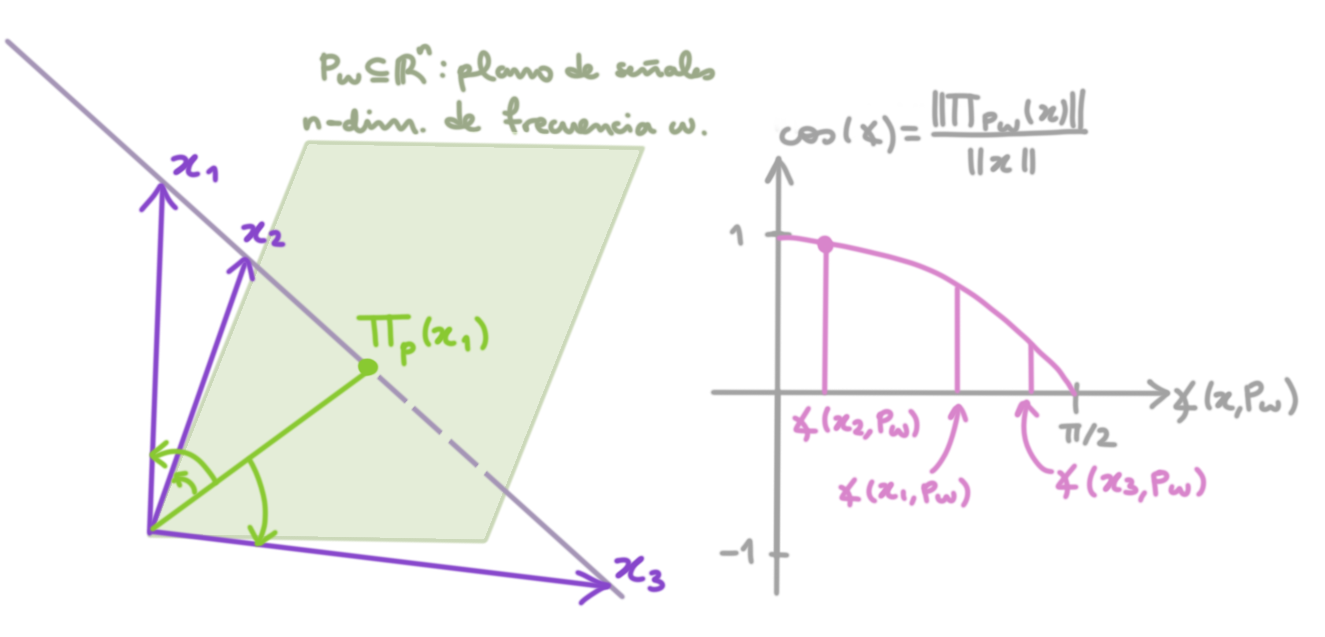
\includegraphics[scale= 1]{20Mar23_1} 
\end{figure}	

Puesto que todas las señales de Legendre discretas
$\mathcal{L}^{n,k}$ tienen norma uno,
\sidenote{En lo que resta de este capítulo, $x$ siempre denotará
a una señal unitaria.}
tenemos la relación simplificada 

\begin{equation}
\label{eq1: 20Mar}
cos \left( \measuredangle (x, W) \right) = || \Pi_{W}(x) || 
\hspace{0.5cm} (x \hspace{0.1cm} \text{unitario).}
\end{equation}

\textbf{Usaremos pues, para dar una medida de qué tanto
reacciona una señal unitaria $x \in \IR^{n}$ a una frecuencia
$\omega >0$ (con $n \nmid \omega$), la norma de la proyección
de $x$ al espacio $P_{\omega} \subseteq \IR^{n}$ 
de señales n-dimensionales de frecuencia $n$.}

Para usar los
resultados expuestos en el apéndice
\ref{ap: Caso particular en el que el subespacio en cuestión es un plano}
conviente establecer una fórmula para
el producto punto entre 
los vectores $f_{n, \omega}$ y $g_{n, \omega}$.
Hacemos esto a continuación.

\begin{prop}
\label{prop: producto punto entre f y g}
Fijados $n \geq 2$ y $\omega \geq 0$, los vectores
$f_{n, \omega}$ y $g_{n, \omega}$, como se definieron
en \eqref{eq5: 19Marzo}
y \eqref{eq6: 19Marzo}, respectivamente, 
son unitarios y linealmente independientes.
Además, 

\begin{equation}
\label{eq9: 19Marzo}
\langle f_{n, \omega} , g_{n, \omega} \rangle =
\frac{\xi_{n, w} \eta_{n, \omega}}{2} \cdot 
\frac{sen(2 \pi \omega)
sen(2 \pi \omega \left( 1- \frac{1}{n} \right))}{sen \left(2 \pi 
\frac{\omega}{n} \right)}
\end{equation}

\end{prop}
\noindent
\textbf{Demostración.}


Aquí usaremos las siguientes tres igualdades:

\begin{equation}
\label{eq10: 19Marzo}
\forall \alpha \in \IR: \hspace{0.2cm}
sen(2 \alpha) = 2 sen(\alpha) cos(\alpha)
\end{equation}



\begin{equation}
\label{eq11: 19Marzo}
\forall z\in \IR: \hspace{0.2cm}
sen(z)= \frac{e^{iz}-e^{-iz}}{2i}
\end{equation}



\begin{equation}
\label{eq12: 19Marzo}
\forall a \in \IR-\{ 1 \}: \hspace{0.2cm}
\suma{\mu=0}{n-1}{a^{r}}= \frac{1-a^{n}}{1-a}.
\end{equation}

\noindent
Tenemos que

\begin{align*}
\langle f_{n,\omega} , g_{n, \omega} \rangle = &
\xi_{n, \omega} \eta_{n, \omega} \langle 
\left( cos (2 \pi \omega \frac{\mu }{n}) \right)_{0 \leq \mu \leq N-1} ,  
\left( cos (2 \pi \omega \frac{\mu }{n}) \right)_{0 \leq \mu \leq N-1} \rangle \\
= & \xi_{n, \omega} \eta_{n, \omega} \suma{\mu=0}{n-1}{
cos (2 \pi \omega \frac{\mu }{n}) sen(2 \pi \omega \frac{\mu }{n})} \\
= & \frac{\xi_{n, \omega} \eta_{n, \omega}}{2}
\suma{\mu=0}{n-1}{
\left( sen(4 \pi \omega \frac{\mu}{n}) \right)} \\
= & \frac{\xi_{n, \omega} \eta_{n, \omega}}{4i} \suma{\mu=0}{n-1}{
\left( e^{4 \pi \omega i \mu/n} - 
e^{-4 \pi \omega i \mu/n} \right) } \\
= & \frac{\xi_{n, \omega} \eta_{n, \omega}}{4i} 
\left(
\frac{1-e^{4 \pi \omega i }}{1-e^{4 \pi \omega i /N}} - 
\frac{1-e^{-4 \pi \omega i }}{1-e^{-4 \pi \omega i /N}} 
\right) \\
= & \frac{\xi_{n, \omega} \eta_{n, \omega}}{4i} 
\left(
\frac{e^{2 \pi \omega i }}{e^{2 \pi \omega i/n }}
\frac{e^{-2 \pi \omega i }-e^{2 \pi \omega i }}{e^{-2 \pi \omega i/n }-e^{2 \pi \omega i /N}} - 
\frac{e^{-2 \pi \omega i }}{e^{-2 \pi \omega i/n }}
\frac{e^{2 \pi \omega i }-e^{-2 \pi \omega i }}{e^{2 \pi \omega i/n }-e^{2 \pi \omega i /N}} 
\right) \\
= & 
\frac{\xi_{n, \omega} \eta_{n, \omega}}{4i} 
\left(
e^{2 \pi \omega i \left( 1-1/n \right)}
\frac{sen(2 \pi \omega)}{sen(2 \pi \omega /n)} - 
e^{-2 \pi \omega i \left( 1-1/n \right)}
\frac{sen(2 \pi \omega)}{sen(2 \pi \omega /n)}
\right) 
\\
= & 
\frac{\xi_{n, \omega} \eta_{n, \omega}}{4i} 
\frac{sen(2 \pi \omega)}{sen(2 \pi \omega /n)}
\left(
e^{2 \pi \omega i \left( 1-1/n \right)} - e^{-2 \pi \omega i \left( 1-1/n \right)}
\right) \\
= &
\frac{\xi_{n, \omega} \eta_{n, \omega}}{4i} 
\frac{sen(2 \pi \omega)}{sen(2 \pi \omega /n)}
\left(
2i \cdot  sen \left( 2 \pi \omega  \left( 1- \frac{1}{n} \right) \right)
\right)\\
= & 
\frac{\xi_{n, \omega} \eta_{n, \omega}}{2} 
\frac{sen(2 \pi \omega)}{sen(2 \pi \omega /n)}
sen \left( 2 \pi \omega  \left( 1- \frac{1}{n} \right) \right). \\
\end{align*}


\QEDB
\vspace{0.2cm}


Podemos ya usar las fórmulas establecidas
en la proposición \ref{prop: formulas 20Marzo}
en nuestra situación particular para llegar a que

\[
 \Pi_{P_{\omega}}(x) = 
\frac{
\langle x, f_{n, \omega} \rangle - \langle f_{n, \omega}, g_{n, \omega} \rangle 
\langle x, g_{n, \omega} \rangle
}
{1-|\langle f_{n, \omega}, g_{n, \omega} \rangle |^{2}  }
f_{n, \omega} +
\frac{
\langle x, g_{n, \omega} \rangle - \langle f_{n, \omega}, g_{n, \omega} \rangle 
\langle x, f_{n, \omega} \rangle
}
{1-|\langle f_{n, \omega}, g_{n, \omega} \rangle |^{2}  }
g_{n, \omega},
\]

\noindent
y

\TODO{Nota que como el ángulo siempre está entre cero y pi/2, el coseno
está entre cero y uno, pero tal vez deberías de considerar un signo que diga
de qué lado del plano se encuentra? No creo que pueda hacer esto, pues para
una dimensión general el plano $P_{\omega}$ no es un hiperplano de $\IR^{n}$...}

\begin{align*}
cos (\measuredangle (x, P_{\omega})) = & || \Pi_{P_{\omega}}(x) ||  \\
= & 
\left(		  
		  \frac{\langle x, f_{n, \omega } \rangle^{2} +  \langle x, g_{n, \omega } \rangle^{2}	
	       -2  \langle x, f_{n, \omega } \rangle^{2} \langle x, g_{n, \omega } \rangle^{2} \langle f_{n, \omega }, g_{n, \omega } \rangle^{2}}{1- \langle f_{n, \omega }, g_{n, \omega } \rangle^{2}}	  
\right) ^{1/2}.
\end{align*}


\begin{defi}
Sean $n \geq 2$ entero, $\omega >0$ con $n \nmid \omega$.
Definimos a la función $\sigma_{n , \omega}: \mathcal{B}_{n}(1) \longrightarrow [0,1]$
\TODO{Pon la notación para la bola unitaria!}
\begin{equation}
\label{eq: def sigmas}
\sigma_{n, \omega}(x) : = 
\left(	
\frac{\langle x, f_{n, \omega } \rangle^{2} +  \langle x, g_{n, \omega } \rangle^{2}	
	       -2  \langle x, f_{n, \omega } \rangle^{2} \langle x, g_{n, \omega } \rangle^{2} \langle f_{n, \omega }, g_{n, \omega } \rangle^{2}}{1- \langle f_{n, \omega }, g_{n, \omega } \rangle^{2}}	  
 \right) ^{1/2},
\end{equation}

\noindent
donde $f_{n, \omega}$ y $g_{n, \omega}$ son como en 
\eqref{eq5: 19Marzo} y \eqref{eq6: 19Marzo}.
\end{defi}


Según todo lo discutido hasta ahora, dado $x \in \IR^{n}$ unitario
y fijada una frecuencia $\omega >0$ con $n \nmid \omega$,
\begin{itemize}
\item si $\sigma_{n, \omega}(x)$ es ``cercano'' a cero, $\omega$ no
es una frecuencia con la que es razonable aproximar a $x$ (pues $x$ será
cercano a ser ortogonal a toda señal de dimensión $n$ y frecuencia 
$\omega$),  mientras que

\item si $\sigma_{n, \omega}(x)$ es ``cercano'' a uno, también es muy cercano
(hablando en términos de distancia euclídea) a su proyección al espacio
$P_{\omega}$, luego $x$ es muy parecido a tener frecuencia $\omega$.
\end{itemize}


\subsection{Buscando el mejor desfase con cierta frecuencia que se ajuste una señal de dimensión $n$}
\TODO{$\omega$ no múltiplo escalar de $n$.}

Dada $x \in \IR^{n}$ unitaria y $\omega > 0$ una frecuencia fija
con $n \nmid \omega$, 
buscamos el desfase $\phi \in [0,1]$ que mejor se ajusta a $x$.

\begin{figure}[H]
	\sidecaption{
	Aquí se grafica una misma señal $x \in \IR^{16}$ y se 
	compara con dos funciones sinusoidales, una con 
	desfase (normalizado) 0.8 y otra con 0.32. Observe que
	la primera parece ajustar mucho mejor la gráfica de $x$.
	\label{fig: ejemplo desfase}
	}
	\centering
	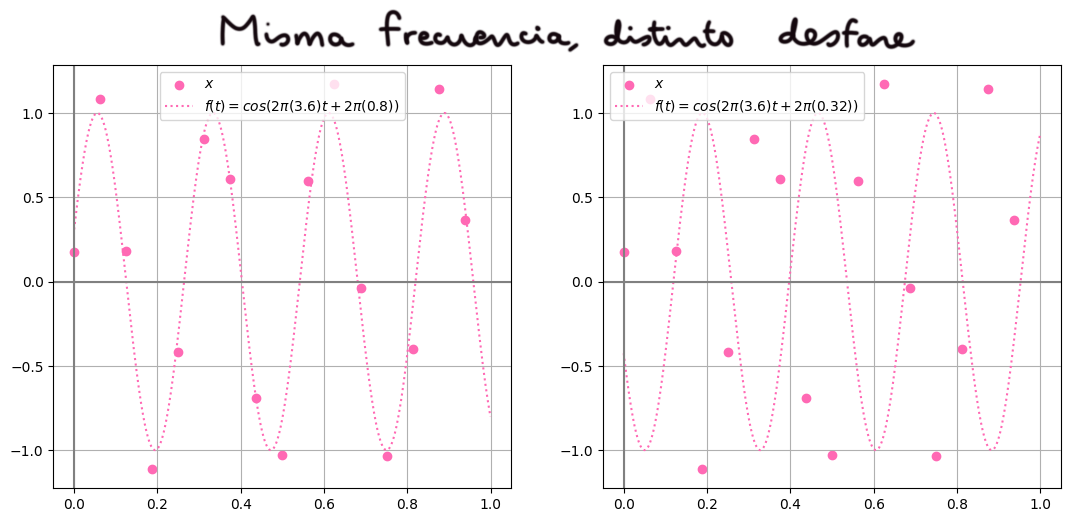
\includegraphics[scale=0.4]{desfase_ejemplo} 
\end{figure}	


Puesto que
$\Pi_{P_{\omega}}(x)$ (donde $P_{\omega}$ es como se definió en 
\eqref{eq2: 20Marzo}) es la señal de frecuencia $\omega$ que está a menor
distancia euclidea de $x$, claro que el desfase $\phi$ buscado es de hecho
el número entre cero y uno tal que 
\[
\Pi_{P_{\omega}}(x) = A (cos(2 \pi \omega t -  2 \pi \phi ))_{t \in I_{n}}
\]
para alguna amplitud $A$.


Como los vectores $f_{n, \omega}$ y $g_{n, \omega}$ 
son linealmente independientes (c.f. observación
\ref{obs: f y g son l.i. y de norma uno}),
podemos usar la ecuación \eqref{eq2: 19Marzo}
para escribir a la proyección de $x$ en $P_{\omega}$ como sigue

\begin{equation}
\label{eq3: 20Marzo}
\Pi_{P_{\omega}}(x)= c (cos (2 \pi \omega t))_{t \in I_{n}} + d 
(sin (2 \pi \omega t))_{t \in I_{n}},
\end{equation}
donde

\begin{equation}
\label{eq4: 20Marzo}
c= \frac{
\langle x, f_{n, \omega} \rangle - \langle f_{n, \omega}, g_{n, \omega} \rangle
\langle x, g_{n, \omega} \rangle
}{1-\langle f_{n, \omega}, g_{n, \omega} \rangle^{2}} \xi_{n, \omega}
\end{equation}
y
\begin{equation}
\label{eq5: 20Marzo}
d= \frac{
\langle x, g_{n, \omega} \rangle - \langle f_{n, \omega}, g_{n, \omega} \rangle
\langle x, f_{n, \omega} \rangle
}{1-\langle f_{n, \omega}, g_{n, \omega} \rangle^{2}} \eta_{n, \omega}.
\end{equation}

\noindent 
Nos conviene más reescribir a \eqref{eq3: 20Marzo} como
\begin{equation}
\label{eq6: 20Marzo}
\Pi_{P_{\omega}}(x)= 
\sqrt{c^{2}+d^{2}}
\left(
C (cos (2 \pi \omega t))_{t \in I_{n}} +
D (sen (2 \pi \omega t))_{t \in I_{n}} 
\right),
\end{equation}

\noindent 
donde

\begin{equation}
\label{eq3: 28Marz23}
C:= \frac{c}{\sqrt{c^{2}+d^{2}}} \hspace{0.2cm} \text{y}
\hspace{0.2cm} D:= \frac{d}{\sqrt{c^{2}+d^{2}}},
\end{equation}

pues, como $C^{2} + D^{2}=1$, existe un único
$\phi \in [0,1]$ tal que
\begin{equation}
\label{eq7: 20Marzo}
C= cos(2 \pi \phi), \hspace{0.2cm} 
D= sin(2 \pi \phi).
\end{equation}

\noindent 
Sustituyendo \eqref{eq7: 20Marzo} en \eqref{eq6: 20Marzo},
llegamos a que

\begin{align*}
\Pi_{P_{\omega}}(x) = & 
\sqrt{c^{2}+d^{2}} \left(
cos(2 \pi \phi) \cdot (cos (2 \pi \omega t))_{t \in I_{n}} +
sin(2 \pi \phi) \cdot (sin (2 \pi \omega t))_{t \in I_{n}} 
\right) \\
= & 
\sqrt{c^{2}+d^{2}} 
((cos(2 \pi \phi) \cdot cos (2 \pi \omega t) +
sin(2 \pi \phi) \cdot sin (2 \pi \omega t) )_{t \in I_{n}} \\
= & 
\sqrt{c^{2}+d^{2}} 
(cos(2 \pi \omega t - 2 \pi \phi))_{t \in I_{n}}.
\end{align*}

\noindent
Además, de \eqref{eq7: 20Marzo} y \eqref{eq7: 20Marzo} 
se deduce que
\begin{equation}
\phi =
\begin{cases}
\frac{tan^{-1}(d/c) }{2 \pi}  \hspace{0.4cm}    \text{   si }   d, c > 0,  \\
\frac{tan^{-1}(d/c) + \pi }{2 \pi} \hspace{0.2cm}  \text{si }  d, c < 0,  \\
\frac{tan^{-1}(d/c) + \pi }{2 \pi} \hspace{0.2cm}  \text{si }  d>0,  c < 0,  \\
\frac{tan^{-1}(d/c) + 2\pi }{2 \pi} \hspace{0.2cm}  \text{si }  d>0,  c < 0. 
\end{cases}
\end{equation}

Hemos probado el siguiente
\begin{teo}
Dados $n \geq 2$, $\omega > 0$ con $n \nmid \omega$ y $x \in \IR^{n}$
unitario, 
\begin{equation}
\label{ec: desfase explicito}
\Pi_{P_{\omega}} (x) = \sqrt{c^{2}+d^{2}} \cdot (
cos (2 \pi \omega t - 2 \pi \phi)
)_{t \in I_{n}} \in \IR^{n},
\end{equation}

\noindent
donde $c$ y $d$ son como en \eqref{eq4: 20Marzo} y 
\eqref{eq5: 20Marzo}, respectivamente, y $\phi$ está 
dado por \eqref{ec: desfase explicito}.
\end{teo}


